\begin{abstract}
\noindent
Quantum controls that agree at the nominal endpoint and in their complete first-order
response to the declared global error coordinates need not have the same finite-error
robustness. We study this residual implementation dependence in a serialized two-atom
Rydberg model---a minimal interacting setting in which amplitude, detuning, and
interaction-calibration responses coexist---with twenty-four control phases and three
global error coordinates.

The main result is a computer-assisted exact-root finite-error ordering theorem. For a
frozen twelve-path cohort, strict 192-bit Krawczyk inclusions certify twelve locally
unique roots whose projective output states and first projective responses exactly match
the reference. Direct outward-rounded Arb propagation of the certified root boxes through
the declared six-axis error functional produces twelve pairwise disjoint performance
intervals, totally ordered according to an order frozen before the propagation, certifying
the complete finite-error ordering for all 66 unordered path pairs. Two computationally
independent mechanism certificates expose the internal structure of this ordering: a
zero-point Taylor jet through order thirty, with formal Cauchy-alias and Dyson-tail
enclosures, certifies 52/66 comparisons with no reversed pair, while the lowest-order
quartic term alone certifies 34/66.

On a separate prospective cohort, a frozen quartic response contraction strongly predicts
the held-out finite-error ranking (Spearman $\rho=0.996992$ on twenty paths), and its
tensor representation is verified to transform covariantly under nonorthogonal
error-coordinate changes. This prospective evidence is not a premise of the theorem. The
theorem is conditional on the declared finite-dimensional model and error functional; it
does not constitute hardware, model-discrepancy, global-fibre, or many-body evidence.
\end{abstract}

\section{Introduction}

Programmable neutral-atom systems expose a rich pulse-level control space, including Rabi
amplitude, phase, detuning, atomic geometry, and Rydberg-mediated
interactions~\cite{silverio2022pulser,henriet2020,saffman2016}. This flexibility permits
many control schedules to realize the same nominal task. It also creates an identification
problem: nominally equivalent implementations can respond differently when calibration
errors are finite.

Endpoint equivalence does not resolve this ambiguity. Even matching the complete
first-order output-state response to the relevant error coordinates may leave a family of
implementations with different higher-order behaviour. The resulting question is not
whether leading errors can be cancelled, but whether the remaining finite-error ordering
can be inferred before those finite-error outcomes are evaluated.

Composite-pulse and dynamically-corrected-gate constructions suppress designated low-order
error
terms~\cite{wimperis1994,kukita2022,barnes2015,khaneja2005,vandersypen2005,khodjasteh2009};
filter-function methods characterize the frequency-domain noise susceptibility of a fixed
control~\cite{green2013}; quantum geometric approaches endow state and parameter manifolds
with the quantum geometric tensor and its curvature~\cite{provost1980}; and
control-landscape theory analyses the critical-point structure of control
objectives~\cite{rabitz2004,chakrabarti2007}. These methods typically optimize or cancel
designated low-order sensitivities of a control. What remains unresolved by these
viewpoints is whether controls that are exactly indistinguishable at the endpoint and
throughout their complete first-order projective response can nevertheless admit a
rigorously certifiable finite-error ordering. Here we condition on that strong
equivalence relation---candidate controls must share both the nominal output state and the
complete first-order output-state response to global amplitude, detuning, and interaction
errors---and study the finite-radius ordering that remains on the implementation fibre,
together with its rigorous certification. We then ask:

\begin{quote}
\sloppy
\emph{Within the remaining implementation fibre, can a zero-error geometric quantity
prospectively predict finite-error robustness, and can that ordering be certified at
locally unique projectively matched controls?}
\end{quote}

This formulation separates two logically distinct tasks. The first is prediction: a local
quantity must be fixed before held-out finite-error evaluation and must rank previously
unseen paths. The second is certification: numerical matching must be replaced by
exact-root existence and uniqueness, and the finite-error ordering must be enclosed by
outward-rounded interval arithmetic, in the validated-numerics tradition of
computer-assisted proof~\cite{lanford1982,tucker2002,vandenberg2015}. High correlation
alone does not provide the second conclusion.

We study a two-atom Rydberg model with twenty-four piecewise-constant phase variables. The
numerical matching Jacobian has rank sixteen, leaving an eight-dimensional numerical
tangent null space that organizes the candidate implementation fibre.

\subsection{Main results}

\textbf{Main theorem (informal statement).} Consider the frozen twelve-path cohort, the
serialized finite-dimensional two-atom Hamiltonian, the declared transverse phase boxes,
and the six-axis mean finite-error functional. For each declared control, a strict Krawczyk
inclusion certifies a locally unique root exactly matched in projective output state and
first projective response. Direct 192-bit outward-rounded Arb propagation over the twelve
certified root boxes produces pairwise disjoint performance intervals whose orientations
agree with the pre-outcome frozen ordering for all $\binom{12}{2}=66$ unordered path pairs.
The formal statements and computer-assisted proofs are given in Theorems~\ref{thm:krawczyk}
and~\ref{thm:ordering}. This result is conditional on the serialized model and declared
error functional; it is not a claim about hardware, model discrepancy, global fibre
topology, or many-body scaling.

\textbf{Mechanism proposition (informal statement).} Over the same certified Krawczyk
boxes, propagation of the zero-point Taylor jet through order thirty, including formal
Cauchy-alias and analytic tail enclosures, certifies 52/66 pairwise comparisons with no
reversed certified pair. This order-thirty calculation is a separate, computationally
distinct mechanism certificate. It is not a premise or computational step in the direct
proof of the main theorem. The formal statement appears in
Proposition~\ref{prop:order30}.

\textbf{Reading guide.} Four quantitative results play different logical roles:
\begin{center}
\begin{tabular}{ll}
66/66 & direct exact-root theorem (main result)\\
52/66 & order-thirty mechanism certificate\\
34/66 & quartic-only boundary\\
$\rho = 0.996992$ & prospective evidence (separate cohort)
\end{tabular}
\end{center}
The frozen order used in the exact-root theorem is supplied by the pre-outcome
order-thirty certificate for the twelve-path cohort; no pathwise identity between the
twenty-path prospective cohort and the twelve-path formal cohort is claimed.

The remainder of the paper follows the logical development from prospective prediction to
exact-root certification. Section~\ref{sec:model} fixes the model and the benchmark error
law; Section~\ref{sec:fibre} defines exact projective response matching and proves a
model-independent quadratic-degeneracy lemma; Section~\ref{sec:quartic} introduces the
prospective quartic predictor; Section~\ref{sec:covariant} constructs its covariant tensor
form; and Section~\ref{sec:certification} certifies locally unique exact projective matched
roots and proves the direct finite-error ordering theorem, together with the separate
order-thirty mechanism certificate.

The result is intentionally model-conditional. It concerns the serialized
finite-dimensional two-atom Hamiltonian, the declared transverse boxes, and the six-axis
mean finite-error functional. It does not establish global fibre topology, worst-case
ranking, many-body scaling, open-system robustness, or hardware-level performance.

\section{Two-atom control model}\label{sec:model}

\subsection{Hamiltonian}

We use the ordered basis
\[
\{\ket{gg},\ket{gr},\ket{rg},\ket{rr}\}.
\]
Let
\[
X_{\Sigma}=X\otimes I+I\otimes X,\qquad
Y_{\Sigma}=Y\otimes I+I\otimes Y,
\]
\[
N_{\Sigma}=n\otimes I+I\otimes n,\qquad N_{rr}=n\otimes n,
\]
where $n=\ket{r}\!\bra{r}$. During segment $j$, the Hamiltonian is
\begin{equation}\label{eq:hamiltonian}
H_{j}(\eps)=\frac{\Omega}{2}(1+\eps_{\Omega})
\bigl(\cos\phi_{j}\,X_{\Sigma}+\sin\phi_{j}\,Y_{\Sigma}\bigr)
-\Omega\,\eps_{\Delta}\,N_{\Sigma}+V(1+\eps_{V})\,N_{rr}.
\end{equation}
The dimensionless error vector is
\[
\eps=(\eps_{\Omega},\eps_{\Delta},\eps_{V}).
\]
The nominal parameters are
\[
\Omega=2\pi\ \mathrm{rad/\mu s},\qquad V=4\Omega,
\]
with 24 segments of duration
\[
\tau=0.1\ \mathrm{\mu s},\qquad T=24\tau=2.4\ \mathrm{\mu s}.
\]
The nominal interaction is represented as $V=C_{6}/R^{6}$. Using the frozen Pulser 1.8.0
\texttt{DigitalAnalogDevice} value $C_{6}=5420158.53$~rad\,$\mu\mathrm{m}^{6}/\mu$s and the
declared $V=4\Omega=8\pi$~rad/$\mu$s gives
\[
R=(C_{6}/V)^{1/6}=7.74394075\ldots\ \mathrm{\mu m}.
\]
This distance is a serialized model parameter rather than a hardware-calibrated
measurement.

The two-atom model is not intended as a many-body approximation. It is a minimal
interacting Rydberg setting in which drive-amplitude, detuning, and interaction-calibration
errors coexist. A single-atom model has no nontrivial $N_{rr}$ response and therefore
cannot represent the three-direction matched response problem studied here.

For a control path
\[
\gamma=(\phi_{1},\ldots,\phi_{24})\in\Tt^{24},
\]
the output state is
\begin{equation}\label{eq:output}
\ket{\psi_{\gamma}(\eps)}=U_{24}(\eps)\cdots U_{2}(\eps)U_{1}(\eps)\ket{gg},
\qquad U_{j}(\eps)=\exp[-i\tau H_{j}(\eps)],
\end{equation}
with time-ordered application from segment 1 to segment 24. All primary calculations use
exact matrix exponentials for the piecewise constant, finite-dimensional model. A
pulse-level emulator was used in an earlier two-atom cross-check, but the formal
certificate in this work is independent of that emulator and does not invoke a cloud
backend. Throughout, \emph{formal certificate} denotes an outward-rounded interval
certificate computed in Arb/ACB ball arithmetic, not a proof-assistant formalization.

\subsection{Loss and held-out error law}

Let $\gamma_{\mathrm{ref}}$ denote the reference schedule and define
\[
\ket{\psi_{\mathrm{ref}}}=\ket{\psi_{\gamma_{\mathrm{ref}}}(0)}.
\]
Two infidelities are used. For the extraction of local response coefficients, the target is
the path-local nominal state,
\begin{equation}\label{eq:iloc}
\Iloc_{\gamma}(\eps)=1-\lvert\braket{\psi_{\gamma}(0)}{\psi_{\gamma}(\eps)}\rvert^{2}.
\end{equation}
For held-out and direct finite-error comparisons, the target is the common reference state,
\begin{equation}\label{eq:iref}
\Iref_{\gamma}(\eps)=1-\lvert\braket{\psi_{\mathrm{ref}}}{\psi_{\gamma}(\eps)}\rvert^{2}.
\end{equation}
At an exact response-matched root, $[\psi_{\gamma}(0)]=[\psi_{\mathrm{ref}}]$ projectively,
so the two definitions coincide; for numerically matched prospective cohorts, they differ
only within the declared matching tolerance. Unless stated otherwise, $\Iref_{\gamma}$ below
denotes~\eqref{eq:iref}.

The held-out error design contains the six signed axial errors
\begin{equation}\label{eq:errorlaw}
E=\{\pm 0.06\,e_{\Omega},\ \pm 0.04\,e_{\Delta},\ \pm 0.05\,e_{V}\}.
\end{equation}
These axis amplitudes define a dimensionless benchmark error law for certificate comparison;
they are not inferred from hardware calibration data. The primary performance functional is
the mean
\begin{equation}\label{eq:meanloss}
\II_{\gamma}=\frac{1}{6}\sum_{\eps\in E}\Iref_{\gamma}(\eps).
\end{equation}
Worst-case infidelity is retained as a secondary diagnostic. The present predictors do not
reliably rank the worst case, and no worst-case theorem is claimed.

\section{Matched implementation fibre}\label{sec:fibre}

\subsection{Endpoint and first-order constraints}

At zero error, remove the unobservable global phase by the path-local horizontal projector
\[
P_{\gamma,\perp}=I-\ket{\psi_{\gamma}(0)}\!\bra{\psi_{\gamma}(0)},
\]
and define the path-local horizontal first-order responses
\begin{equation}\label{eq:jresponse}
J_{\gamma,a}=P_{\gamma,\perp}\,
\frac{\partial}{\partial\eps_{a}}\ket{\psi_{\gamma}(\eps)}\bigg|_{\eps=0},
\qquad a\in\{\Omega,\Delta,V\}.
\end{equation}
Since $\psi_{\gamma}(0)$ and $\psi_{\mathrm{ref}}$ agree only up to a global phase, align
them before comparison by the common phase factor
\begin{equation}\label{eq:phasealign}
c_{\gamma}=\frac{\braket{\psi_{\mathrm{ref}}}{\psi_{\gamma}(0)}}
{\lvert\braket{\psi_{\mathrm{ref}}}{\psi_{\gamma}(0)}\rvert}\in U(1),
\qquad \widetilde{J}_{\gamma,a}=c_{\gamma}J_{\gamma,a},
\end{equation}
and compare the phase-aligned response $\widetilde{J}_{\gamma,a}$ with
$J_{\mathrm{ref},a}$.

\begin{definition}[Numerically matched implementation fibre]\label{def:fibre}
For a declared tolerance $\eta_{F}$, the numerical matched fibre $\Ff_{\eta}$ consists of
controls $\gamma$ satisfying
\begin{equation}\label{eq:fibre}
\II_{\gamma}(0)\le\eta,\qquad
\lVert \widetilde{J}_{\gamma,a}-J_{\mathrm{ref},a}\rVert\le\eta,
\quad a\in\{\Omega,\Delta,V\},
\end{equation}
with $\widetilde{J}_{\gamma,a}$ the phase-aligned response of Eq.~\eqref{eq:phasealign}.
\end{definition}

\subsection{Exact projective constraint map}

The dynamics preserves the exchange-symmetric three-dimensional subspace. In a fixed
symmetric basis we write the state as
\[
\psi=(\psi_{0},\psi_{1},\psi_{2})^{T}\in\Cc^{3},
\]
and eliminate the unobservable global phase by the projective coordinates
\begin{equation}\label{eq:chart}
w_{c}=\frac{\psi_{c}}{\psi_{0}},\qquad c=1,2,
\end{equation}
valid on any region where the chart denominator $\psi_{0}$ excludes zero. For each error
direction $a\in\{\Omega,\Delta,V\}$, the induced projective first response is
\begin{equation}\label{eq:projresp}
\dot{w}_{a,c}=\frac{\dot{\psi}_{a,c}\,\psi_{0}-\psi_{c}\,\dot{\psi}_{a,0}}{\psi_{0}^{2}},
\qquad c=1,2,
\end{equation}
where $\dot{\psi}_{a}=\partial_{\eps_{a}}\psi\bigr|_{\eps=0}$. The exact constraint map is
then
\begin{equation}\label{eq:constraintmap}
F(\boldsymbol{\phi})=
\resizebox{0.72\textwidth}{!}{$\displaystyle
\begin{pmatrix}
\Re(w-w_{\mathrm{ref}})\\
\Im(w-w_{\mathrm{ref}})\\
\Re(\dot{w}_{\Omega}-\dot{w}_{\Omega,\mathrm{ref}})\\
\Im(\dot{w}_{\Omega}-\dot{w}_{\Omega,\mathrm{ref}})\\
\Re(\dot{w}_{\Delta}-\dot{w}_{\Delta,\mathrm{ref}})\\
\Im(\dot{w}_{\Delta}-\dot{w}_{\Delta,\mathrm{ref}})\\
\Re(\dot{w}_{V}-\dot{w}_{V,\mathrm{ref}})\\
\Im(\dot{w}_{V}-\dot{w}_{V,\mathrm{ref}})
\end{pmatrix}$}
\in\Rr^{16}.
\end{equation}
The exact matching used below is therefore exact projective output-state and
first-projective-response matching: it is exact after elimination of the global phase,
rather than a componentwise equality of raw state vectors. The numerical optimizer retains
the full phase-aligned complex output state and the three full phase-aligned complex state
tangents; redundant real components are retained in the residual vector, while
singular-value decomposition determines the independent rank.

\subsection{Quadratic degeneracy under first-response matching}

The next lemma is model-independent. It upgrades the empirical agreement of quadratic loss
coefficients to an exact statement: projective first-response matching forces two families
to share the same quadratic loss form, so their symmetrized losses can first differ at
fourth order.

\begin{lemma}[Quadratic degeneracy under projective first-response matching]%
\label{lem:quadratic}
Let $\psi_{\alpha}(\eps)$ and $\psi_{\beta}(\eps)$ be normalized analytic state families in
a finite-dimensional Hilbert space such that
\[
[\psi_{\alpha}(0)]=[\psi_{\beta}(0)]=[\psi_{0}]
\]
projectively, with identical horizontal first derivatives at the origin,
$h_{\alpha,a}=h_{\beta,a}$, where
\[
h_{\gamma,a}=P_{\perp}\,
\frac{\partial}{\partial\eps_{a}}\ket{\psi_{\gamma}(\eps)}\bigg|_{\eps=0},
\qquad P_{\perp}=I-\ket{\psi_{0}}\!\bra{\psi_{0}}.
\]
Then
\[
\bigl(1-\lvert\braket{\psi_{0}}{\psi_{\alpha}(\eps)}\rvert^{2}\bigr)
-\bigl(1-\lvert\braket{\psi_{0}}{\psi_{\beta}(\eps)}\rvert^{2}\bigr)
=\Or(\lVert\eps\rVert^{3}),
\]
and for the symmetrized losses of Eq.~\eqref{eq:symmetric},
\[
S_{\alpha}(t,v)-S_{\beta}(t,v)=\Or(t^{4}).
\]
\end{lemma}

\begin{proof}
The infidelity is invariant under a global phase, so after phase alignment we may take
$\psi_{\alpha}(0)=\psi_{\beta}(0)=\psi_{0}$ and use the common target $\psi_{0}$. Write
$f_{\gamma}(\eps)=1-\lvert\braket{\psi_{0}}{\psi_{\gamma}(\eps)}\rvert^{2}$ and expand
\[
\braket{\psi_{0}}{\psi_{\gamma}(\eps)}
=1+\eps_{a}A_{a}+\tfrac{1}{2}\eps_{a}\eps_{b}A_{ab}+\Or(\lVert\eps\rVert^{3}),
\]
with $A_{a}=\braket{\psi_{0}}{\partial_{a}\psi_{\gamma}}$ and
$A_{ab}=\braket{\psi_{0}}{\partial_{a}\partial_{b}\psi_{\gamma}}$ evaluated at $\eps=0$;
repeated indices are summed. Differentiating the normalization
$\braket{\psi_{\gamma}}{\psi_{\gamma}}=1$ gives $\Re A_{a}=0$ and
$\Re A_{ab}=-\Re\braket{\partial_{a}\psi_{\gamma}}{\partial_{b}\psi_{\gamma}}$. The linear
term of $f_{\gamma}$ therefore vanishes, and its quadratic term is the Fubini--Study form
of the horizontal derivatives,
\[
f_{\gamma}(\eps)=g_{ab}\,\eps_{a}\eps_{b}+\Or(\lVert\eps\rVert^{3}),
\qquad g_{ab}=\Re\braket{h_{\gamma,a}}{h_{\gamma,b}},
\]
since $h_{\gamma,a}=\partial_{a}\psi_{\gamma}-A_{a}\psi_{0}$. Identical horizontal first
derivatives give $g^{\alpha}_{ab}=g^{\beta}_{ab}$, hence
$f_{\alpha}-f_{\beta}=\Or(\lVert\eps\rVert^{3})$. Symmetrization in $t$ cancels the
odd-order terms, so the difference of the symmetric responses starts at order $t^{4}$.
\end{proof}

\subsection{Dimension count and generation}

The control has 24 phase variables. At the reference solution, the numerical constraint
Jacobian has rank
\[
\rank DF(\gamma_{\mathrm{ref}})=16,
\]
leaving an eight-dimensional numerical null space that organizes the candidate
implementation fibre. Candidate paths are generated by:
\begin{enumerate}[itemsep=0.1em]
\item drawing a seeded direction in the numerical null space;
\item applying a finite displacement;
\item projecting back to the constraint set by nonlinear least squares;
\item rejecting candidates whose constraint residual or pairwise phase distance fails a
predeclared gate.
\end{enumerate}
No held-out finite-error outcome is evaluated during candidate generation. The maximum
constraint residual in the reported runs is of order $10^{-11}$.

\begin{remark}[Global fibre versus local certified roots]\label{rem:globalfibre}
The numerical rank and residual establish a highly accurate computational fibre, suggesting
a locally eight-dimensional numerical implementation fibre, not the exact existence of a
global eight-dimensional solution manifold. A complete global fibre theorem would require a
square transverse formulation and a global interval-Newton or Krawczyk proof. The present
work instead establishes 12 locally unique roots exactly matched in projective output state
and first projective response via strict Krawczyk inclusions in transverse boxes. The
global fibre structure remains open.
\end{remark}

Figure~\ref{fig:schematic} summarizes the local mechanism. The drawing is schematic: it
represents one local chart and does not assert that the twelve certified roots belong to
one globally connected exact fibre. The geometric object used below is the quartic response
tensor of the loss, not a curvature tensor of a chosen connection or metric.

\begin{figure}[t]
\centering
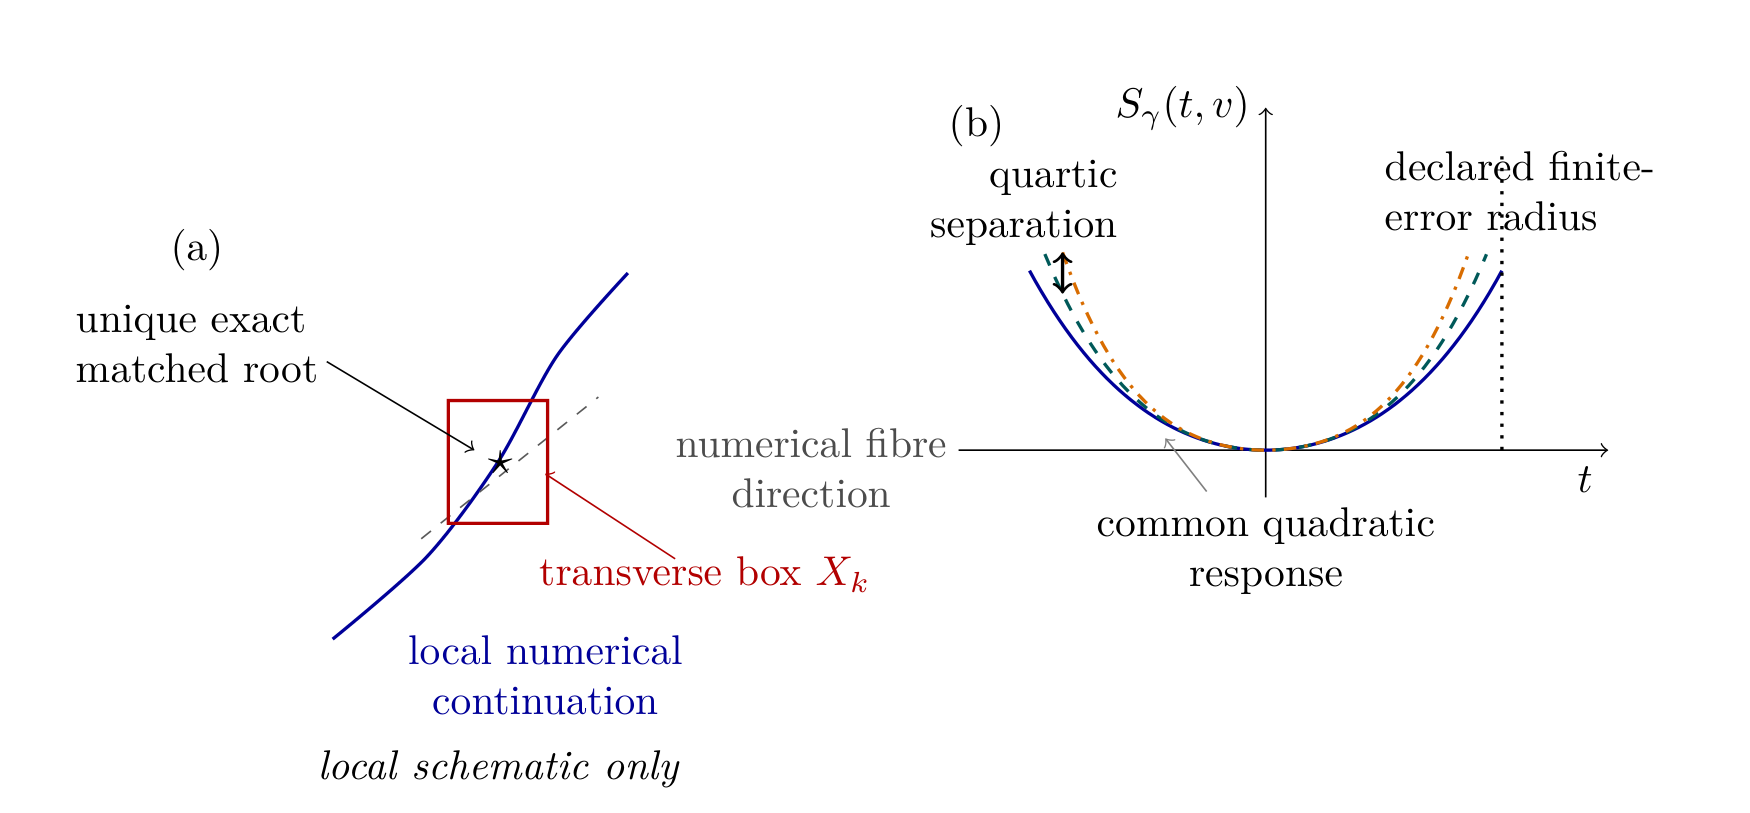
\includegraphics[width=0.9\textwidth]{fig1.png}
\caption{Schematic of local response matching and quartic separation. (a) In a local
control-space chart, the projective output-state and first-response constraints define
numerical tangent directions; the formal certificate establishes a unique exact matched
root only inside each declared transverse box and does not assert a global connected fibre.
(b) Exact projective first-response matching makes the quadratic loss form common.
Symmetrized finite-error responses can therefore first separate through their quartic
coefficients. The tensor $\Aa^{(4)}$ is a fourth-order response susceptibility, not a
Riemannian curvature tensor.}
\label{fig:schematic}
\end{figure}
